% !TeX root=../main.tex
% Insert with % !TeX root=../main.tex
% Insert with % !TeX root=../main.tex
% Insert with % !TeX root=../main.tex
% Insert with \input{./tex/chapter3_walk_dependencies} at the start of 3.3.4
% after finalizing the computational procedures.
% Requires only TikZ, graphicx, xcolor and XePersian (already loaded).
\begin{figure}[!htbp]
\centering
\begin{LTR}
\centering
\resizebox{0.94\linewidth}{!}{%
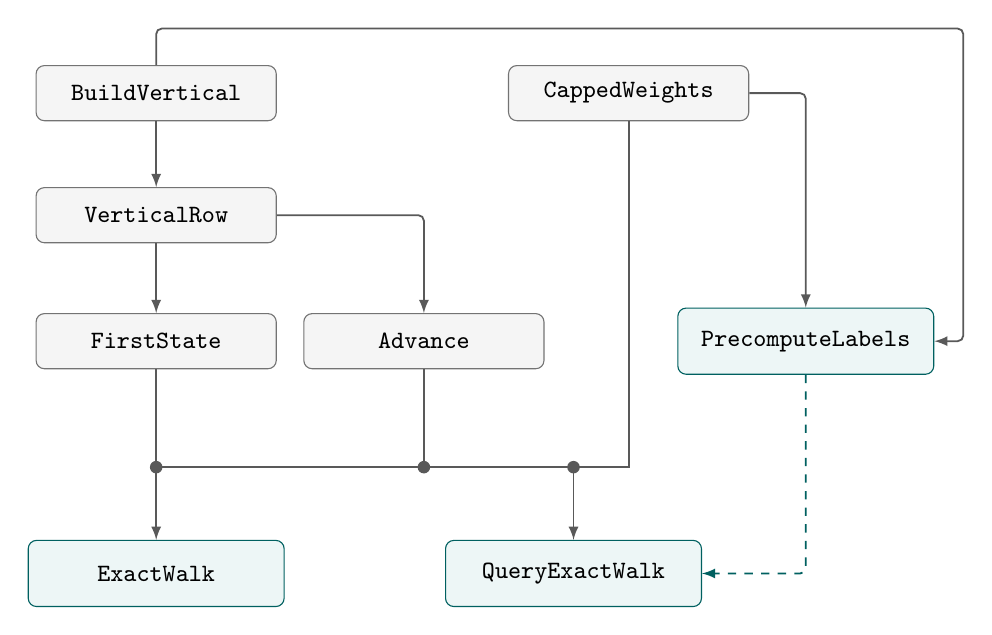
\begin{tikzpicture}[
    x=1cm,y=1cm,
    helper/.style={draw=black!55,fill=black!4,rounded corners=3pt,
        minimum width=3.05cm,minimum height=0.70cm,
        inner sep=4pt,font=\small\ttfamily,align=center},
    procedure/.style={helper,draw=teal!75!black,fill=teal!7,
        minimum width=3.25cm,minimum height=0.84cm},
    dependency/.style={->,>=latex,draw=black!65,line width=0.65pt,
        rounded corners=2pt},
    wire/.style={draw=black!65,line width=0.65pt},
    optional/.style={dependency,dashed,draw=teal!75!black},
    junction/.style={circle,fill=black!65,inner sep=1.6pt}
]
    % Preparation and reusable subroutines.
    \node[helper] (build) at (2.0,0) {BuildVertical};
    \node[helper] (weights) at (8.0,0) {CappedWeights};
    \node[helper] (vertical) at (2.0,-1.55) {VerticalRow};
    \node[helper] (first) at (2.0,-3.15) {FirstState};
    \node[helper] (advance) at (5.4,-3.15) {Advance};

    % Main procedures.
    \node[procedure] (precompute) at (10.25,-3.15) {PrecomputeLabels};
    \node[procedure] (exact) at (2.0,-6.1) {ExactWalk};
    \node[procedure] (query) at (7.3,-6.1) {QueryExactWalk};

    % The arrow points from a provider to a consumer.
    \draw[dependency] (build.south) -- (vertical.north);
    \draw[dependency] (vertical.south) -- (first.north);
    \draw[dependency] (vertical.east) -| (advance.north);
    % PrecomputeLabels uses the base vertical rows directly,
    % not the forward Advance routine.
    \draw[dependency] (build.north) -- (2.0,0.82)
        -- (12.25,0.82) |- (precompute.east);
    \draw[dependency] (weights.east) -| (precompute.north);

    % Shared dependencies of both forward-walk procedures:
    % FirstState, Advance and CappedWeights.
    \draw[wire] (first.south) -- (2.0,-4.75);
    \draw[wire] (advance.south) -- (5.4,-4.75);
    \draw[wire] (weights.south) -- (8.0,-4.75) -- (2.0,-4.75);
    \node[junction] at (5.4,-4.75) {};
    \node[junction] at (7.3,-4.75) {};
    \node[junction] at (2.0,-4.75) {};
    \draw[dependency] (2.0,-4.75) -- (exact.north);
    \draw[dependency] (7.3,-4.75) -- (query.north);
    % The shared precomputed matrix is optional for the query.
    \draw[optional] (precompute.south) |- (query.east);
\end{tikzpicture}%
}
\end{LTR}
\caption{ساختار وابستگی زیرروال‌ها و روندهای محاسبهٔ امید گشت.
پیکان‌ها از زیرروال یا روند فراهم‌کنندهٔ اطلاعات به مصرف‌کنندهٔ آن
رسم شده‌اند. خط‌چین نشان‌دهندهٔ استفادهٔ اختیاری از ماتریس
پیش‌محاسبه‌شده در روند استنتاج است؛ در صورت استفاده از این ماتریس،
انتشار پیش‌رونده و محاسبهٔ دوبارهٔ ضرایب گشت برای نمونهٔ جدید
ضروری نیست.}
\label{cmp:fig:ch3-walk-procedure-dependencies}
\end{figure}
 at the start of 3.3.4
% after finalizing the computational procedures.
% Requires only TikZ, graphicx, xcolor and XePersian (already loaded).
\begin{figure}[!htbp]
\centering
\begin{LTR}
\centering
\resizebox{0.94\linewidth}{!}{%
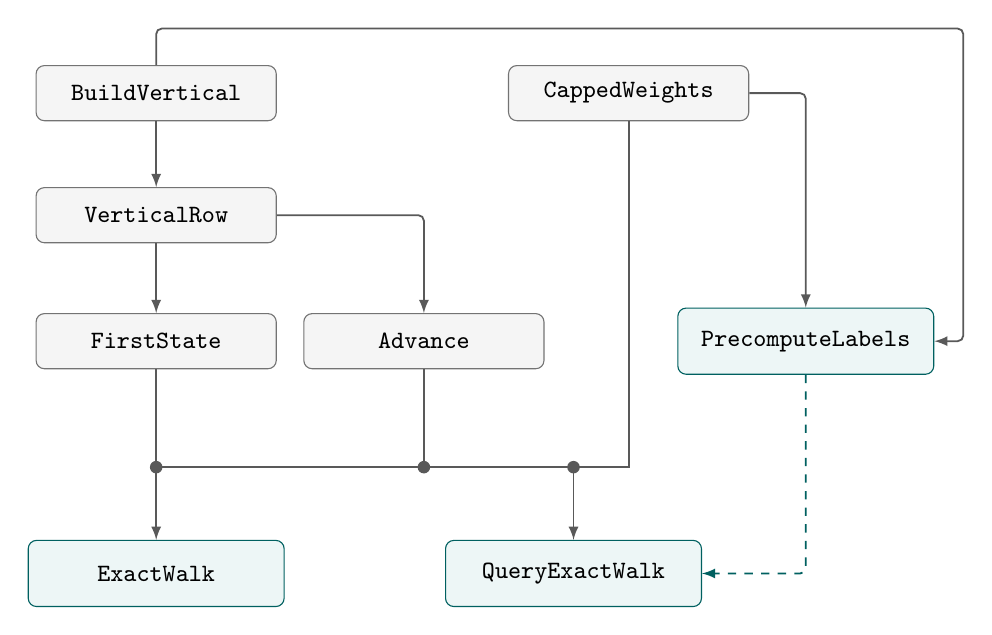
\begin{tikzpicture}[
    x=1cm,y=1cm,
    helper/.style={draw=black!55,fill=black!4,rounded corners=3pt,
        minimum width=3.05cm,minimum height=0.70cm,
        inner sep=4pt,font=\small\ttfamily,align=center},
    procedure/.style={helper,draw=teal!75!black,fill=teal!7,
        minimum width=3.25cm,minimum height=0.84cm},
    dependency/.style={->,>=latex,draw=black!65,line width=0.65pt,
        rounded corners=2pt},
    wire/.style={draw=black!65,line width=0.65pt},
    optional/.style={dependency,dashed,draw=teal!75!black},
    junction/.style={circle,fill=black!65,inner sep=1.6pt}
]
    % Preparation and reusable subroutines.
    \node[helper] (build) at (2.0,0) {BuildVertical};
    \node[helper] (weights) at (8.0,0) {CappedWeights};
    \node[helper] (vertical) at (2.0,-1.55) {VerticalRow};
    \node[helper] (first) at (2.0,-3.15) {FirstState};
    \node[helper] (advance) at (5.4,-3.15) {Advance};

    % Main procedures.
    \node[procedure] (precompute) at (10.25,-3.15) {PrecomputeLabels};
    \node[procedure] (exact) at (2.0,-6.1) {ExactWalk};
    \node[procedure] (query) at (7.3,-6.1) {QueryExactWalk};

    % The arrow points from a provider to a consumer.
    \draw[dependency] (build.south) -- (vertical.north);
    \draw[dependency] (vertical.south) -- (first.north);
    \draw[dependency] (vertical.east) -| (advance.north);
    % PrecomputeLabels uses the base vertical rows directly,
    % not the forward Advance routine.
    \draw[dependency] (build.north) -- (2.0,0.82)
        -- (12.25,0.82) |- (precompute.east);
    \draw[dependency] (weights.east) -| (precompute.north);

    % Shared dependencies of both forward-walk procedures:
    % FirstState, Advance and CappedWeights.
    \draw[wire] (first.south) -- (2.0,-4.75);
    \draw[wire] (advance.south) -- (5.4,-4.75);
    \draw[wire] (weights.south) -- (8.0,-4.75) -- (2.0,-4.75);
    \node[junction] at (5.4,-4.75) {};
    \node[junction] at (7.3,-4.75) {};
    \node[junction] at (2.0,-4.75) {};
    \draw[dependency] (2.0,-4.75) -- (exact.north);
    \draw[dependency] (7.3,-4.75) -- (query.north);
    % The shared precomputed matrix is optional for the query.
    \draw[optional] (precompute.south) |- (query.east);
\end{tikzpicture}%
}
\end{LTR}
\caption{ساختار وابستگی زیرروال‌ها و روندهای محاسبهٔ امید گشت.
پیکان‌ها از زیرروال یا روند فراهم‌کنندهٔ اطلاعات به مصرف‌کنندهٔ آن
رسم شده‌اند. خط‌چین نشان‌دهندهٔ استفادهٔ اختیاری از ماتریس
پیش‌محاسبه‌شده در روند استنتاج است؛ در صورت استفاده از این ماتریس،
انتشار پیش‌رونده و محاسبهٔ دوبارهٔ ضرایب گشت برای نمونهٔ جدید
ضروری نیست.}
\label{cmp:fig:ch3-walk-procedure-dependencies}
\end{figure}
 at the start of 3.3.4
% after finalizing the computational procedures.
% Requires only TikZ, graphicx, xcolor and XePersian (already loaded).
\begin{figure}[!htbp]
\centering
\begin{LTR}
\centering
\resizebox{0.94\linewidth}{!}{%
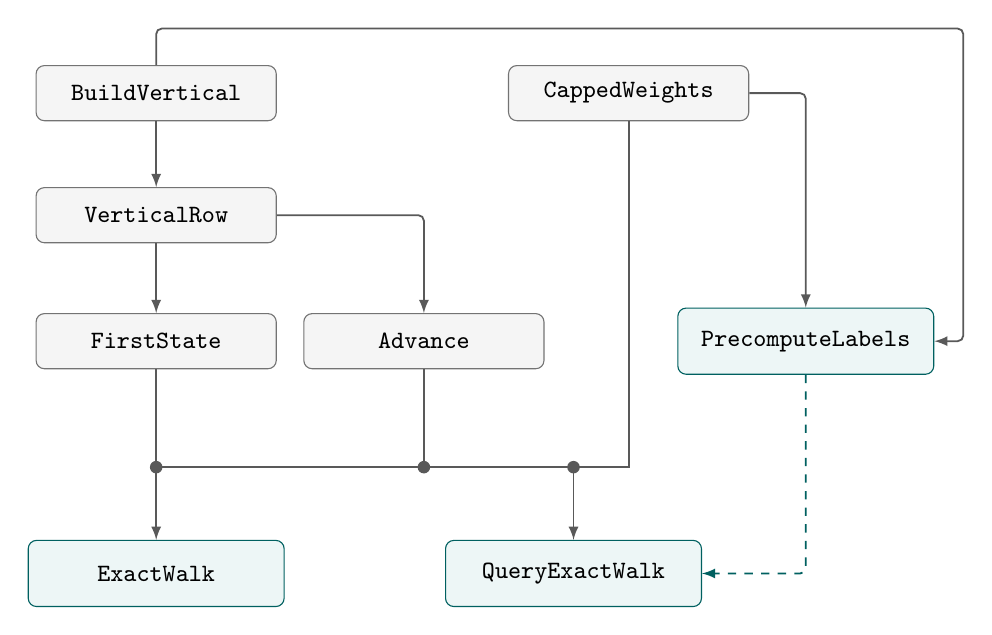
\begin{tikzpicture}[
    x=1cm,y=1cm,
    helper/.style={draw=black!55,fill=black!4,rounded corners=3pt,
        minimum width=3.05cm,minimum height=0.70cm,
        inner sep=4pt,font=\small\ttfamily,align=center},
    procedure/.style={helper,draw=teal!75!black,fill=teal!7,
        minimum width=3.25cm,minimum height=0.84cm},
    dependency/.style={->,>=latex,draw=black!65,line width=0.65pt,
        rounded corners=2pt},
    wire/.style={draw=black!65,line width=0.65pt},
    optional/.style={dependency,dashed,draw=teal!75!black},
    junction/.style={circle,fill=black!65,inner sep=1.6pt}
]
    % Preparation and reusable subroutines.
    \node[helper] (build) at (2.0,0) {BuildVertical};
    \node[helper] (weights) at (8.0,0) {CappedWeights};
    \node[helper] (vertical) at (2.0,-1.55) {VerticalRow};
    \node[helper] (first) at (2.0,-3.15) {FirstState};
    \node[helper] (advance) at (5.4,-3.15) {Advance};

    % Main procedures.
    \node[procedure] (precompute) at (10.25,-3.15) {PrecomputeLabels};
    \node[procedure] (exact) at (2.0,-6.1) {ExactWalk};
    \node[procedure] (query) at (7.3,-6.1) {QueryExactWalk};

    % The arrow points from a provider to a consumer.
    \draw[dependency] (build.south) -- (vertical.north);
    \draw[dependency] (vertical.south) -- (first.north);
    \draw[dependency] (vertical.east) -| (advance.north);
    % PrecomputeLabels uses the base vertical rows directly,
    % not the forward Advance routine.
    \draw[dependency] (build.north) -- (2.0,0.82)
        -- (12.25,0.82) |- (precompute.east);
    \draw[dependency] (weights.east) -| (precompute.north);

    % Shared dependencies of both forward-walk procedures:
    % FirstState, Advance and CappedWeights.
    \draw[wire] (first.south) -- (2.0,-4.75);
    \draw[wire] (advance.south) -- (5.4,-4.75);
    \draw[wire] (weights.south) -- (8.0,-4.75) -- (2.0,-4.75);
    \node[junction] at (5.4,-4.75) {};
    \node[junction] at (7.3,-4.75) {};
    \node[junction] at (2.0,-4.75) {};
    \draw[dependency] (2.0,-4.75) -- (exact.north);
    \draw[dependency] (7.3,-4.75) -- (query.north);
    % The shared precomputed matrix is optional for the query.
    \draw[optional] (precompute.south) |- (query.east);
\end{tikzpicture}%
}
\end{LTR}
\caption{ساختار وابستگی زیرروال‌ها و روندهای محاسبهٔ امید گشت.
پیکان‌ها از زیرروال یا روند فراهم‌کنندهٔ اطلاعات به مصرف‌کنندهٔ آن
رسم شده‌اند. خط‌چین نشان‌دهندهٔ استفادهٔ اختیاری از ماتریس
پیش‌محاسبه‌شده در روند استنتاج است؛ در صورت استفاده از این ماتریس،
انتشار پیش‌رونده و محاسبهٔ دوبارهٔ ضرایب گشت برای نمونهٔ جدید
ضروری نیست.}
\label{cmp:fig:ch3-walk-procedure-dependencies}
\end{figure}
 at the start of 3.3.4
% after finalizing the computational procedures.
% Requires only TikZ, graphicx, xcolor and XePersian (already loaded).
\begin{figure}[!htbp]
\centering
\begin{LTR}
\centering
\resizebox{0.94\linewidth}{!}{%
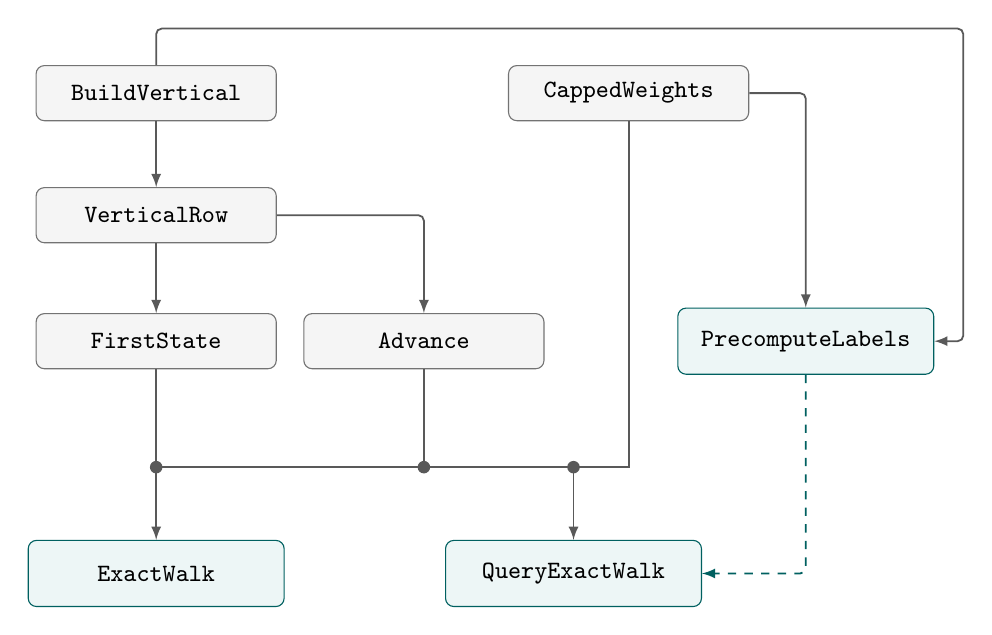
\begin{tikzpicture}[
    x=1cm,y=1cm,
    helper/.style={draw=black!55,fill=black!4,rounded corners=3pt,
        minimum width=3.05cm,minimum height=0.70cm,
        inner sep=4pt,font=\small\ttfamily,align=center},
    procedure/.style={helper,draw=teal!75!black,fill=teal!7,
        minimum width=3.25cm,minimum height=0.84cm},
    dependency/.style={->,>=latex,draw=black!65,line width=0.65pt,
        rounded corners=2pt},
    wire/.style={draw=black!65,line width=0.65pt},
    optional/.style={dependency,dashed,draw=teal!75!black},
    junction/.style={circle,fill=black!65,inner sep=1.6pt}
]
    % Preparation and reusable subroutines.
    \node[helper] (build) at (2.0,0) {BuildVertical};
    \node[helper] (weights) at (8.0,0) {CappedWeights};
    \node[helper] (vertical) at (2.0,-1.55) {VerticalRow};
    \node[helper] (first) at (2.0,-3.15) {FirstState};
    \node[helper] (advance) at (5.4,-3.15) {Advance};

    % Main procedures.
    \node[procedure] (precompute) at (10.25,-3.15) {PrecomputeLabels};
    \node[procedure] (exact) at (2.0,-6.1) {ExactWalk};
    \node[procedure] (query) at (7.3,-6.1) {QueryExactWalk};

    % The arrow points from a provider to a consumer.
    \draw[dependency] (build.south) -- (vertical.north);
    \draw[dependency] (vertical.south) -- (first.north);
    \draw[dependency] (vertical.east) -| (advance.north);
    % PrecomputeLabels uses the base vertical rows directly,
    % not the forward Advance routine.
    \draw[dependency] (build.north) -- (2.0,0.82)
        -- (12.25,0.82) |- (precompute.east);
    \draw[dependency] (weights.east) -| (precompute.north);

    % Shared dependencies of both forward-walk procedures:
    % FirstState, Advance and CappedWeights.
    \draw[wire] (first.south) -- (2.0,-4.75);
    \draw[wire] (advance.south) -- (5.4,-4.75);
    \draw[wire] (weights.south) -- (8.0,-4.75) -- (2.0,-4.75);
    \node[junction] at (5.4,-4.75) {};
    \node[junction] at (7.3,-4.75) {};
    \node[junction] at (2.0,-4.75) {};
    \draw[dependency] (2.0,-4.75) -- (exact.north);
    \draw[dependency] (7.3,-4.75) -- (query.north);
    % The shared precomputed matrix is optional for the query.
    \draw[optional] (precompute.south) |- (query.east);
\end{tikzpicture}%
}
\end{LTR}
\caption{ساختار وابستگی زیرروال‌ها و روندهای محاسبهٔ امید گشت.
پیکان‌ها از زیرروال یا روند فراهم‌کنندهٔ اطلاعات به مصرف‌کنندهٔ آن
رسم شده‌اند. خط‌چین نشان‌دهندهٔ استفادهٔ اختیاری از ماتریس
پیش‌محاسبه‌شده در روند استنتاج است؛ در صورت استفاده از این ماتریس،
انتشار پیش‌رونده و محاسبهٔ دوبارهٔ ضرایب گشت برای نمونهٔ جدید
ضروری نیست.}
\label{cmp:fig:ch3-walk-procedure-dependencies}
\end{figure}
